%%%%%%%%%%%%%%%%%%%%%%%%%%%%%%%%%%%%%%%%%%%%%%%%%%%%%%%%%%%%%%%%%%%%%%%%%%%%%%%%
\chapter{Identifying Relevant Expressions}\label{sec:etl}

\begin{chapterBody}

\begin{figure}[ht]
    \centering
    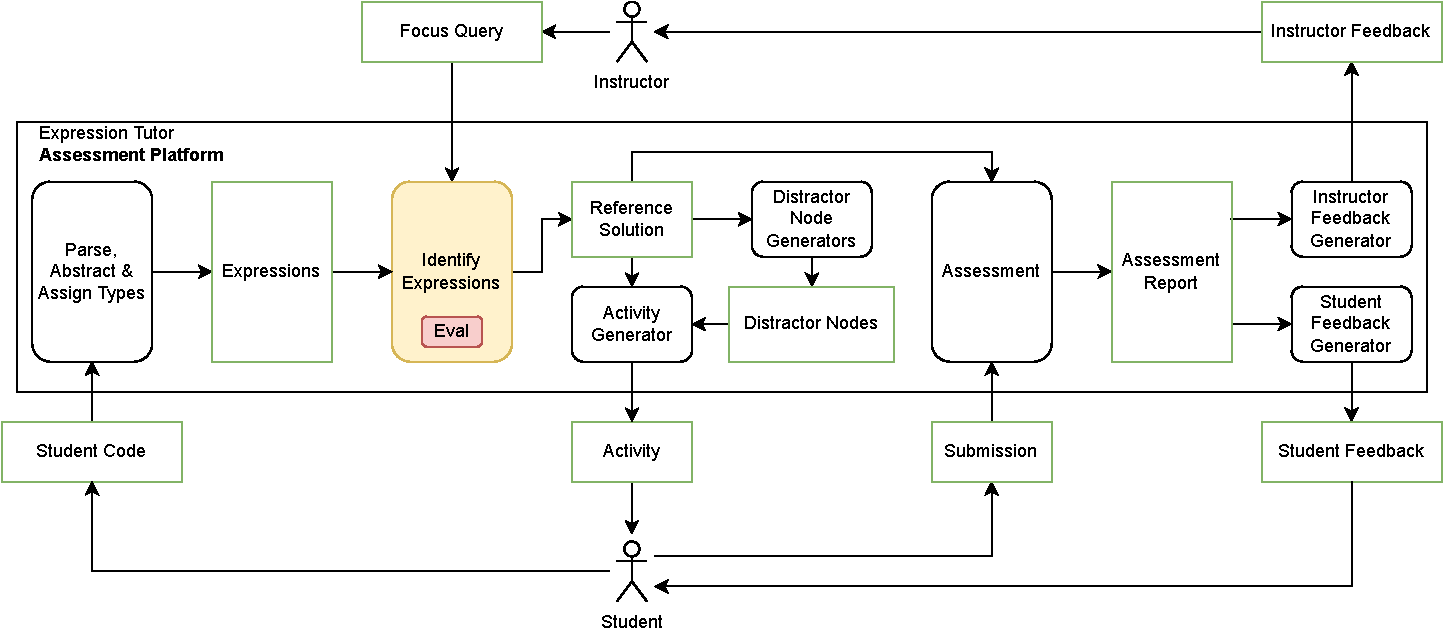
\includegraphics[width=\textwidth]{res/4/et_loop_etl.pdf}
    \caption{Identify relevant Expressions in a code–base given a focus query.}
    \label{fig:etl-intro-loop}
\end{figure}

To automatically generate activities from students' code, there must
be a process to select one or more expressions that serve as the basis.
The instructor has to be able to specify a particular learning goal.
One such example of a learning goal could be \textit{Given a description of
the shape and contents of a (single or multi-dimensional) array, write an
expression using an array initializer to allocate and initialize that array.}
To find code in student's submissions that corresponds to the learning
goal, we need to use some code–querying tool. Such a tool would, given
a \textit{focus query} and a code–base, identify a number of expressions
that matched.

Formally, we need to devise a function that takes a focus query and a
code–base and returns a set of expressions, as highlighted in
\textbf{Figure~\ref{fig:etl-intro-loop}}.

\[
\text{expressionSelection}:
\left(\text{FocusQuery}, \text{List}[\text{Expression}]\right)
\rightarrow
\text{Set}\left[\text{Expression}\right]
\]

\section{Code–Querying Tools}

We look at some of the most popular existing code–querying tools and
evaluate them.

\subsection{X–Path Based Solutions}

There exists different tools that can parse source code and allow to query the
AST using X–Path strings as queries. Notable examples of such tools are PMD
(Programming Mistakes Detector) and srcML\@.

The Programming Mistakes Detector (PMD) tool is an ``extensible cross-language
static code analyzer'' written in Java~\cite{copeland_pmd_2002}.
This powerful tool not only comes with a large number of built-in rules that
can check given source code against a number of well–known design flaws, but
it allows the user to specify custom rules to find \textit{patterns} in source
code. This is achieved by supplying X–Path strings as a query.

On the other hand, the \texttt{srcML} program adopts the srcML format. It
consists of an XML representation for source code (\citet{collard_srcml_2016}).
In this XML document, the markup tags identify elements of the abstract syntax
tree (AST) for the language. The usage of the XML format allows to take
advantage of existing XML tools to perform exploration, analysis, and 
manipulation of source code, such as X–Path for querying nodes of the AST\@.

X–Path allows to query XML semi–structured data: both in the case of PMD and
srcML, the tool would first parse the source code for an Abstract Syntax Tree
(AST) of the Java and then represent it as an XML document.
This approach allows to tap into the great ecosystem of tooling built around
the XML document format, but presents a few drawbacks for the specific use–case
of querying expression trees.
One problem we would encounter with this approach is that X–Path favours a
linear (\textit{path}–like) matching process.
When matching tree patterns, it is often necessary to not only look at
\textit{parent}–\textit{child} node relationships, but also at node
\textit{siblings}.
While this is also doable in X–Path, the complexity of the query strings
increases considerably (\citet{goos_xpath_2002}).

It is also important to note that both PMD and srcML support just a limited
set of languages that may or may not match those that the Expression Tutor
platform wants to support.

Finally, the fact that these tools rely on the AST data structure, makes
queries harder to handle. Writing queries requires the user to have deep
understanding of the language and names of its various constructs.

As an example, if we wanted to query for a simple Java expression that contains
a division between two integers. The query should be able to match expressions
such as \lstinline{1 / 2}, \lstinline{a / 2} (assuming \texttt{a} is an
integer variable), \lstinline{1 + a / 2} and \lstinline{1 + a / (a + 2)}.
The PMD query that achieves this would be the one shown in
\textbf{Listing~\ref{lst:et-xpath-query-example}}. While it clearly
a powerful tool, by looking at the example for a query for a simple expression,
it is apparent how X–Path based solution are not easy to use for someone who
does not have extensive knowledge about them.

\begin{lstlisting}[label={lst:et-xpath-query-example},
                   caption={X–Path query for PMD. This query looks for
                            expressions that contain a division between
                            two integers.},
                   language=xpath]
//*[@Expression='true']/../(*[@Expression='true'] | .)//InfixExpression[@Operator='/' and pmd-java:typeIs('int')]/*[@Expression='true' and pmd-java:typeIs('int')]/following-sibling::*[@Expression='true' and pmd-java:typeIs('int')]/ancestor::*[@Expression='true']
\end{lstlisting}

\subsection{SemGrep}

SemGrep, which stands for \textit{Semantic Grep}, is a \textit{``fast,
lightweight, polyglot, open source static analysis tool to find bugs and
enforce code standards''}~\cite{padioleau_semgrep_2021}.
It operates by using queries written in a Domain Specific Language (DSL) that is
made of code patterns that look like regular code.

Even tough the promise of querying source code using ``source–code–like''
patterns is very appealing, there is one important limitation.
The actual implementation of this feature, in SemGrep, is specific for each one
of the multiple supported programming languages.
The upside of having language–specific implementations of these DSL–based 
``code search engines'' is that they allow for interesting features such as
\textit{meta–variables} that enable interesting advanced query behaviors such
as conditional selection based on evaluated values.
On the other hand, having different language–specific implementations other
than increasing the maintenance cost for preserving feature parity across all
languages, it may also require the syntax of the DSL itself to vary depending
on the reserved keywords and symbols of each supported programming language.

\subsection{Comparison \& Considerations}

By looking at the key features of each solution, as described in the previous
section and summarized in \textbf{Table~\ref{tab:etl-cqt-compare}}, it is 
apparent how none of them perfectly suits our needs of being able to easily
query expressions. In particular, all of them perform matches and report
``root nodes'', rather than being able to match sub–expressions and report back
the bigger parent expression. This is extremely important to avoid all
the different expression selected from different code–bases with a single query
to be very similar and the respective expression trees small.

\begin{table}[ht]
\centering
\begin{tabular}{l|lll}
                & \thead{srcML} & \thead{PMD}   & \thead{SemGrep} \\\hline
\textbf{Syntax} & XML           & XML           & SemGrep DSL \\
\textbf{Format} & AST–based     & AST–based     & Token–based \\
\textbf{Supported Languages}
                & Polyglot      & Polyglot      & Polyglot \\
\textbf{Query targets}
                & Any construct & Any construct & Any construct \\
\textbf{Queries on tree–shaped structures} & Complex (X–Path) &
Complex (X–Path) & Possible \\
\end{tabular}
\caption{Comparison between srcML, PMD and SemGrep.}
\label{tab:etl-cqt-compare}
\end{table}

To this end, we design and implement a DSL specifically to query expressions
trees, avoiding the shortcomings of the other solutions in this niche.
Rather than directly querying for expressions in source code, we leverage the 
existing functionalities that allow the extraction and conversion of
expressions from code to expression trees. Then, by reducing the scope in
which the DSL operates, all the required operations may be accomplished more
easily. Moreover, this query language can also serve as a DSL that can represent
the Expression as Tree notional machine in a purely textual form.

\section{Expression Tree Language}\label{sec:etl-grammar}

Expression Tree Language (ETL) is a DSL designed to easily represent and query
expression trees. Just like the expression tree diagrams introduced in
Section~\ref{sec:bg-rw-le-et}, it is completely language–agnostic and any
well–formed tree represented by an expression tree diagram can convert to an
\textit{ETL tree} without loss of information.
The language agnosticism enables more powerful workflows such as support for
querying for expressions in a polyglot project, as long as there exists a 
conversion from the source code files to expression tree diagrams.

While expression trees are simple to write on a free–form medium such as paper
or on a whiteboard, they are more difficult to easily represent with just a
mouse and a keyboard. Drawing an expression tree on the Expression Tutor
website consists of a complex sequence of actions involving different input
devices, making drawing a more complex tree a time–consuming task.

This language design takes inspiration from hand–drawn expression trees and 
adopts some regular expressions tokens (such as \texttt{?}, \texttt{+} and
\texttt{|}). The syntax of this DSL is parenthetical, inspired by LISP–style
programming languages.
Rather than focusing on complex and advanced representations, a few simple
features are included to make ETL expressions easy to both understand and write.
The target audience for this DSL are instructors who want to either query for
expressions in code–bases or want to easily represent some expression tree in
a coincise way.

\subsection{Base Constructs}

These constructs allow to build concrete expression trees that can also
convert to expression tree diagrams.

\subsubsection*{Forest}

A Forest is a collection of nodes. 

\begin{minipage}{.33\textwidth}
A forest with 3 empty nodes.
\end{minipage}
\begin{minipage}{.33\textwidth}
\begin{lstlisting}[language=etl]
( ) ( ) ( )
\end{lstlisting} 
\end{minipage}
\begin{minipage}{.33\textwidth}
\includegraphics[height=2em]{res/4/etd_forest.png}
\end{minipage}

\subsubsection*{Node}

A node contains any number of \textit{NodeContentElement}s between two
parentheses. Nodes can have optional types. To specify the type of a node,
it is necessary to append the colon (\texttt{:}) character and the name of the 
type after the parenthesis that \textit{closes} the node.
This construct corresponds to the Node construct of the expression tree
diagram (detailed in Section~\ref{sec:bg-et-etd}).

\begin{minipage}{.3\linewidth}
An empty node.
\end{minipage}
\hspace{.02\linewidth}
\begin{minipage}{.3\linewidth}
\begin{lstlisting}[language=etl]
( )
\end{lstlisting} 
\end{minipage}
\hspace{.02\linewidth}
\begin{minipage}{.3\linewidth}
\includegraphics[height=2em]{res/4/etd_node_empty.png}
\end{minipage}

\begin{minipage}{.3\linewidth}
A typed node (type \texttt{int}) \hfill\break
containing the text ``1''.
\end{minipage}
\hspace{.02\linewidth}
\begin{minipage}{.3\linewidth}
\begin{lstlisting}[language=etl]
("1"): int
\end{lstlisting} 
\end{minipage}
\hspace{.02\linewidth}
\begin{minipage}{.3\linewidth}
\includegraphics[height=3em]{res/4/etd_node_with_type.png}
\end{minipage}

\subsubsection*{NodeContentElem}

A node content element is a construct found inside a Node.

\begin{itemize}
    \item \textbf{NameDef}: To represent a name definition element, we write a
string enclosed by double quotes and preceded by the character \texttt{d}.
This construct corresponds to the NameDef construct of the expression tree
diagram (Section~\ref{sec:bg-et-etd}).

\begin{minipage}{.3\linewidth}
A node with a nameDef of ``myVar''.
\end{minipage}
\hspace{.02\linewidth}
\begin{minipage}{.3\linewidth}
\begin{lstlisting}[language=etl]
(d"myVar")
\end{lstlisting} 
\end{minipage}
\hspace{.02\linewidth}
\begin{minipage}{.3\linewidth}
\includegraphics[height=2em]{res/4/etd_node_name_def.png}
\end{minipage}

    \item \textbf{NameUse}: To represent a name use element, we write a string
enclosed by double quotes and preceded by the character \texttt{u}.
This construct corresponds to the NameUse construct of the expression tree
diagram (Section~\ref{sec:bg-et-etd}).

\begin{minipage}{.3\linewidth}
A node with a nameUse of ``myVar''.
\end{minipage}
\hspace{.02\linewidth}
\begin{minipage}{.3\linewidth}
\begin{lstlisting}[language=etl]
(u"myVar")
\end{lstlisting} 
\end{minipage}
\hspace{.02\linewidth}
\begin{minipage}{.3\linewidth}
\includegraphics[height=2em]{res/4/etd_node_name_use.png}
\end{minipage}

    \item \textbf{Other}: To represent an Other element, we write a string
enclosed by double quotes. This construct corresponds to the Other construct of 
the expression tree diagram (Section~\ref{sec:bg-et-etd}). 

\begin{minipage}{.3\linewidth}
A node with an Other representing the ``+'' character.
\end{minipage}
\hspace{.02\linewidth}
\begin{minipage}{.3\linewidth}
\begin{lstlisting}[language=etl]
("+")
\end{lstlisting} 
\end{minipage}
\hspace{.02\linewidth}
\begin{minipage}{.3\linewidth}
\includegraphics[height=2em]{res/4/etd_node_name_other.png}
\end{minipage}

    \item \textbf{Node}: A Node can also be a node content element, indicating
that such a node is a child of the containing (parent) node. The syntax remains
unchanged.

\begin{minipage}{.3\linewidth}
A parent node with a child node.
\end{minipage}
\hspace{.02\linewidth}
\begin{minipage}{.3\linewidth}
\begin{lstlisting}[language=etl]
("parent" ("child"))
\end{lstlisting} 
\end{minipage}
\hspace{.02\linewidth}
\begin{minipage}{.3\linewidth}
\includegraphics[height=4em]{res/4/etd_node_child.png}
\end{minipage}
\end{itemize}

\subsection{Query–Exclusive Constructs}

The following are \texttt{NodeContentElement} constructs that may only be found
inside a query node. They can only be used for building an ETL query and their
usage makes the ETL Forest impossible to convert to an expression tree diagram.

\begin{itemize}
    \item \textbf{Hole}: To represent an unconnected Hole, we write an
open parenthesis immediately followed by a close parenthesis \texttt{()}. This
construct corresponds to the Hole  construct of the expression tree diagram
(Section~\ref{sec:bg-et-etd}).

\begin{minipage}{.3\linewidth}
A node with one \hfill\break
unconnected hole.
\end{minipage}
\hspace{.02\linewidth}
\begin{minipage}{.3\linewidth}
\begin{lstlisting}[language=etl]
( () )
\end{lstlisting} 
\end{minipage}
\hspace{.02\linewidth}
\begin{minipage}{.3\linewidth}
\includegraphics[height=2em]{res/4/etd_node_hole.png}
\end{minipage}

    \item \textbf{Alternative}: To represent an Alternative element, we write
the vertical bar character \texttt{|}, and offers an alternative between the
two surrounding elements. To offer more than two choices, it is possible to
use consecutively multiple alternative elements.

\begin{minipage}{.3\linewidth}
A query node for a node with either ``a'' or ``b''
followed by the element ``c''.
\end{minipage}
\hspace{.02\linewidth}
\begin{minipage}{.3\linewidth}
\begin{lstlisting}[language=etl]
("a" | "b"  "c")
\end{lstlisting} 
\end{minipage}
\hspace{.02\linewidth}
\begin{minipage}{.3\linewidth}
\includegraphics[height=2em]{res/4/etd_query_alt_1.png}
\end{minipage}

\begin{minipage}{.3\linewidth}
A query node for a node with any either ``a'', ``b'' or a hole as its
single element.
\end{minipage}
\hspace{.02\linewidth}
\begin{minipage}{.3\linewidth}
\begin{lstlisting}[language=etl]
("a" | "b" | ())
\end{lstlisting}
\end{minipage}
\hspace{.02\linewidth}
\begin{minipage}{.3\linewidth}
\includegraphics[height=2em]{res/4/etd_query_alt_2.png}
\end{minipage}
    
    \item \textbf{Any}: To represent an Any element, we write the underscore
character \texttt{\_}. This element matches any single 
\texttt{NodeContentElement} regardless of type or contents.

\begin{minipage}{.3\linewidth}
A query node for a node with one single content element.
\end{minipage}
\hspace{.02\linewidth}
\begin{minipage}{.3\linewidth}
\begin{lstlisting}[language=etl]
(_)
\end{lstlisting} 
\end{minipage}
\hspace{.02\linewidth}
\begin{minipage}{.3\linewidth}
\includegraphics[height=2em]{res/4/etd_query_any.png}
\end{minipage}

    \item \textbf{RegEx}: To represent a regular expression element, we write
a string enclosed by forward slashes \texttt{/}.
We use this element to match against a single textual node content
element (\texttt{Other}, \texttt{NameDef} and \texttt{NameUse} elements) which
content matches the regular expression defined within the forward slashes.

\begin{minipage}{.3\linewidth}
A query node for a node with a single content element that matches the
regular expression
\texttt{[A-Z]\{3\}-[0-9]\{2\}}
\end{minipage}
\hspace{.02\linewidth}
\begin{minipage}{.3\linewidth}
\begin{lstlisting}[language=etl]
(/[A-Z]{3}-[0-9]{2}/)
\end{lstlisting} 
\end{minipage}
\hspace{.02\linewidth}
\begin{minipage}{.3\linewidth}
\includegraphics[height=2em]{res/4/etd_query_reg.png}
\end{minipage}

    \item \textbf{Optional}: To represent an Optional element, we append
the question mark character \texttt{?} to another element.
It symbolizes that the previous element may or may not be matched.

\begin{minipage}{.3\linewidth}
A query node for a node containing an ``a'' element, optionally 
followed by a ``b'' element.
\end{minipage}
\hspace{.02\linewidth}
\begin{minipage}{.3\linewidth}
\begin{lstlisting}[language=etl]
("a" "b"?)
\end{lstlisting} 
\end{minipage}
\hspace{.02\linewidth}
\begin{minipage}{.3\linewidth}
\includegraphics[height=2em]{res/4/etd_query_opt.png}
\end{minipage}

    \item \textbf{Plus}: To represent the Plus element, we append the plus
character \texttt{+} to another element. It symbolizes that the previous element will be matched one or more times.

\begin{minipage}{.3\linewidth}
A query node for a node containing an ``a'' element, followed by one
or more ``b'' elements.
\end{minipage}
\hspace{.02\linewidth}
\begin{minipage}{.3\linewidth}
\begin{lstlisting}[language=etl]
("a" "b"+)
\end{lstlisting} 
\end{minipage}
\hspace{.02\linewidth}
\begin{minipage}{.3\linewidth}
\includegraphics[height=2em]{res/4/etd_query_plus.png}
\end{minipage}

    \item \textbf{Star}: To represent the Star element, we append the star
character \texttt{*}.  It symbolizes that the previous element will be matched zero or more times.

\begin{minipage}{.3\linewidth}
A query node for a node containing an ``a'' element, followed by zero
or more ``b'' elements.
\end{minipage}
\hspace{.02\linewidth}
\begin{minipage}{.3\linewidth}
\begin{lstlisting}[language=etl]
("a" "b"*)
\end{lstlisting} 
\end{minipage}
\hspace{.02\linewidth}
\begin{minipage}{.3\linewidth}
\includegraphics[height=2em]{res/4/etd_query_star.png}
\end{minipage}

    \item \textbf{Group}: To represent the Group element and its contents,
we write a sequence of \hfill\break
\texttt{NodeContentElement}s enclosed between the square brackets characters
\texttt{[]}. This element is useful to apply other query elements such as
Alternatives, Optional, Plus and Star to many elements instead of just one at
the same time.

\begin{minipage}{.3\linewidth}
A query node for a node containing an ``a'' element, optionally followed
by both the elements ``b'' and ``c''.
\end{minipage}
\hspace{.02\linewidth}
\begin{minipage}{.3\linewidth}
\begin{lstlisting}[language=etl]
("a" ["b" "c"]?)
\end{lstlisting} 
\end{minipage}
\hspace{.02\linewidth}
\begin{minipage}{.3\linewidth}
\includegraphics[height=2em,]{res/4/etd_query_grp.png}
\end{minipage}
\end{itemize}

\textbf{Listing~\ref{lst:etl-grammar}} details the grammar specification
for the Expression Tree Language written in Backus Normal Form (BNF).

\subsection{Implementation}\label{sec:etl-impl}

To make use of ETL to query for expressions in code–bases, it is necessary to
implement a query algorithm. For any given pair of expression tree diagram
and ETL Query node, the algorithm returns a boolean value. This value
indicates whether the given diagram matches the query.

Formally, we need to devise a function that takes an expression tree diagram
and an ETL Query and tests whether the Query matches in the given expression
tree diagram.

\[
\text{match}:
\left( \text{ExprTreeDiagram}, \text{EtlQuery}\right)
\rightarrow
\text{Boolean}
\]

We implement this algorithm as a combination between tree–matching and
regex–matching algorithms.
The algorithm starts by converting the expression tree diagram to an ETL tree.
If the input diagram is not a valid tree, then this conversion fails and
the algorithm reports that there was no match for that specific diagram.
Performing tree–structure based queries on diagrams that are not valid trees
is not ideal as it can easily yield inconsistent results due to the difference
in the relationships between nodes in the two data structures.

Once the input diagram has been converted to an \textit{input tree}, it is
possible to make use of tree–matching techniques, during which, by walking the
two trees, we try to establish whether the query tree is (or is a subset of)
the input tree.

Unlike in common tree–matching algorithms, the content of the nodes presents
yet another dimension for our algorithm to perform a match. Each node contains
a number of node content elements and we can think of each one of them as a
character in a plain textual regular expression. Some characters are literals
(Other, NameUse and NameDef), other have special meanings. Some are identical
to regex tokens, such as the alternative (\texttt{|}), the optional
(\texttt{?}) and the repeat (\texttt{*} and \texttt{+}).

To perform this regex–like matching, we adopt the classic strategy of
\textit{converting} the regular expression into a deterministic finite
automaton (DFA) and applying the algorithm devised by
\citet{thompson_programming_1968} to verify whether the content of a node
matches the contents in the respective node of the query tree. In particular,
the concrete implementation takes inspiration from Henry Spencer's Regex
library~\cite{schumacher_software_1994}. The Regular expression, or rather,
the sequence of NodeContentElem from the query node, is transformed into a list
of instruction for a virtual machine (VM) that interprets and run them against
another sequence of  NodeContentElem (this time originating from the ``input''
node).
Henry Spencer's VM can execute 5 different instructions that may compose its
programs:

\begin{enumerate}
    \item \texttt{elem $x$}: Match a single element $x$. In the case of textual
regex, this is a character, while for ETL this is a node content element.
    \item \texttt{jump $x$}: Set the program counter (PC) of the VM to the
instruction at $x$.
    \item \texttt{split $x1$ $x2$}: Fork the current \textit{thread} and
continue its execution at $x2$, while the original thread continues at $x1$.
    \item \texttt{mark $x$}: Marks the opening of a group if the given value
$x$ is even, or the closing of a group if the value of $x$ is odd (for the
group that was opened at $x-1$). This is used to check whether all groups have
completely been matched by the time the execution completes.
    \item \texttt{match}: Report successful matching if there is no open group.
\end{enumerate}

Other than these 5 instructions, we introduce another one to satisfy the needs
of our ETL query matching algorithm:

\begin{enumerate}
    \item[6.] \texttt{child $x$}: This instruction calls back to the 
\textit{tree matching part} of the algorithm to attempt to continue the
matching on a child node $x$ before proceeding with the parent. If the
contents of the child node are not successfully matched, then the parent's
matching also fail.
\end{enumerate}

\textbf{Table~\ref{tab:etl-lang-to-vm}} showcases how the different Expression
Tree Language query constructs are converted to VM instructions.
\textbf{Listing~\ref{lst:etl-query-algo}} provides the pseudo–code implementation
of the ETL query matching algorithm described in this section.

When all nodes in the ETL query have been completely matched against the input
diagram, the algorithm reports a successful correspondence, otherwise, the
query is performed again on all sub–trees of the input diagram until either one
correspondence is found or all nodes have been used as input root and no
correspondence was found.

\begin{table}[ht]
\centering
\begin{tabular}{llll}
\thead{Name} & \thead{ETL query} & \thead{VM instructions} &
\thead{FSM} \\\hline
Alternative & 
\begin{lstlisting}[language=etl]
("a" | "b")
\end{lstlisting} &
\begin{lstlisting}[language=etl-vm]
0: split 1 3
1: elem "a"
2: jump 4
3: elem "b"
4: match
\end{lstlisting} &
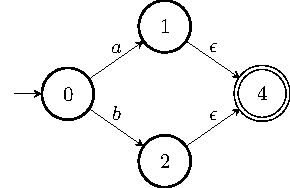
\includegraphics[width=0.3\linewidth]{res/4/etl_vm_alt.pdf} \\

Optional &
\begin{lstlisting}[language=etl]
("a"?)
\end{lstlisting} &
\begin{lstlisting}[language=etl-vm]
0: split 1 2
1: elem "a"
2: match
\end{lstlisting} &
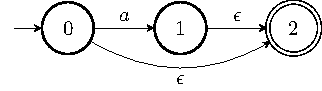
\includegraphics[width=0.3\linewidth]{res/4/etl_vm_opt.pdf} \\

Plus &
\begin{lstlisting}[language=etl]
("a"+)
\end{lstlisting} &
\begin{lstlisting}[language=etl-vm]
0: elem "a"
1: split 0 2
2: match
\end{lstlisting} &
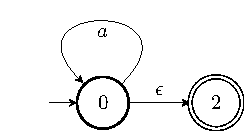
\includegraphics[width=0.3\linewidth]{res/4/etl_vm_plus.pdf} \\

Star &
\begin{lstlisting}[language=etl]
("a"*)
\end{lstlisting} &
\begin{lstlisting}[language=etl-vm]
0: split 1 3
1: elem "a"
2: jump 0
3: match
\end{lstlisting} &
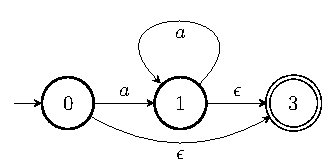
\includegraphics[width=0.3\linewidth]{res/4/etl_vm_star.pdf} \\

Child &
\begin{lstlisting}[language=etl]
("a" ("b"))
\end{lstlisting} &
\begin{lstlisting}[language=etl-vm]
0: elem "a"
1: child 1
2: match
\end{lstlisting} & - \\

Hole &
\begin{lstlisting}[language=etl]
( () )
\end{lstlisting} &
\begin{lstlisting}[language=etl-vm]
0: child 0
1: match
\end{lstlisting} & - \\

Group (with plus) &
\begin{lstlisting}[language=etl]
(["a" "b"]+)
\end{lstlisting} &
\begin{lstlisting}[language=etl-vm]
0: mark 0
1: elem "a"
2: elem "b"
3: mark 1
4: split 0 5
5: match
\end{lstlisting} & - \\
\end{tabular}
\caption{Language constructs to VM instructions.}
\label{tab:etl-lang-to-vm}
\end{table}

\section{Evaluation}\label{sec:etl-eval}

In this section we evaluate the capabilities of the Expression Tree Language
by showcasing how it is possible to represent any expression of the Java 
programming language (at version 11). To do so, we take the ``exhaustive and
unambiguous definition of expression constructs in Java'' devised by
\citet{chiodini_expressions_2022} and reproduce all expression definitions using
ETL queries. By doing so, we demonstrate that it is indeed possible to utilize
this DSL to represent any expression of a complex programming language such as
Java.

For each expression construct defined in the Java language specification
(JLS) we provide a brief description, the ``expression structure'' as defined
by the grammar and the equivalent ``ETL Query''.
In the expression structure we make use of some \textit{meta–variables} to
simplify the grammar rules. These are the same found in Table~1~and~2 of
\cite{chiodini_expressions_2022} and are reported here as well for ease
of access (\textbf{Table~\ref{tab:etl-eval-java-metavar}}).

\begin{table}[ht]
\centering
\begin{tabular}{lll}
\thead{Meta–Variable} & \thead{Meaning} & \thead{JLS} \\
$ T $                & Any Type                     & 4.1 \\
$ T_r $              & Reference Type               & 4.3 \\
Block                & Code Block                   & 4.2 \\
ArrayInit            & Array Initializer            & 10.6 \\
Id                   & Identifier                   & 3.8 \\
Params               & Lambda Parameters            & 15.27.1 \\
AssignOp             & Assignment Operator          & 15.26 \\
PostfixOp            & Postfix Operator             & 15.14 \\ 
PrefixOp             & Unary Operator (except cast) & 15.15 \\
InfixOp              & Binary Operator (except \texttt{instanceof}) 
                     & 15.[17-24] \\
IntegerLiteral       & Integer Literal              & 3.10.1 \\
FloatingPointLiteral & Floating–Point Literal       & 3.10.2 \\
CharacterLiteral     & Character Literal            & 3.10.4 \\
StringLiteral        & String Literal               & 3.10.5 \\
\end{tabular}
\caption{Meaning of the \textit{meta–variables} used to simplify the Java grammar
rules written in this section. Taken from~\cite{chiodini_expressions_2022}}
\label{tab:etl-eval-java-metavar}
\end{table}

\subsection*{Class Instance Creation (JLS \S15.9)}

A class instance creation expression specifies the class to be instantiated,
followed by type arguments (if the instantiated class has a parametric 
type) and by the list of the actual value arguments to the constructor.
\vspace{1em}

\begin{minipage}[t]{.45\linewidth}
\textbf{Expression Structure} \hfill\break
\texttt{
[$e$.] {\color{bp-blue}new}
\hfill\break\hspace*{0.5em}
[{\color{bp-blue}<}$T$ \{, $T$\}{\color{bp-blue}>}]
\hfill\break\hspace*{0.5em}
Tr{\color{bp-blue}(}[$e$\{,$e$\}]{\color{bp-blue})}[Block]
} \\ 
\end{minipage}
\begin{minipage}[t]{.45\linewidth}
\textbf{ETL Query}
\begin{lstlisting}[language=etl]
([() "."]? "new" 
 ["<" /\w+/ ["," /\w+/]* ">"]?
 /\w+/ "(" () ["," ()]* ")" "..."?)
\end{lstlisting}
\end{minipage}

\subsection*{This Expression (JLS \S15.8.3)}

When used as a primary expression, the \texttt{this} keyword denotes a
reference to the object which invokes the instance method.
\vspace{1em}

\begin{minipage}[t]{.45\linewidth}
\textbf{Expression Structure} \hfill\break
\texttt{[$T_r$.]{\color{bp-blue}this}}
\end{minipage}
\begin{minipage}[t]{.45\linewidth}
\textbf{ETL Query}
\begin{lstlisting}[language=etl]
(()? "this")
\end{lstlisting}
\end{minipage}

\subsection*{Variable}

\noindent\textbf{Simple Variable Access (JLS \S6.5.6.1)}

An identifier that represents a bound name of a local variable, parameter
field accessible at the point at which the identifier occurs.
\vspace{1em}

\begin{minipage}[t]{.45\linewidth}
\textbf{Expression Structure} \hfill\break
\texttt{Id}
\end{minipage}
\begin{minipage}[t]{.45\linewidth}
\textbf{ETL Query}
\begin{lstlisting}[language=etl]
(/\w+/)
\end{lstlisting}
\end{minipage}

\noindent\textbf{Field Access (JLS \S15.11)}

A field access expression may access the field of an object, a reference to
which is the value of an expression.
\vspace{1em}

\begin{minipage}[t]{.45\linewidth}
\textbf{Expression Structure} \hfill\break
\texttt{[($e$|$T_r$).]Id}
\end{minipage}
\begin{minipage}[t]{.45\linewidth}
\textbf{ETL Query}
\begin{lstlisting}[language=etl]
([[() | /\w+/] "."]* /\w+/)
\end{lstlisting}
\end{minipage}

\begin{lstlisting}[language=etl]
\end{lstlisting}

\noindent\textbf{Super Field Access (JLS \S15.11.2)}

A super field access expression may access the field of an object, a reference
to which is the value of the \texttt{super} keyword.
\vspace{1em}

\begin{minipage}[t]{.45\linewidth}
\textbf{Expression Structure} \hfill\break
\texttt{[$T_r$.]{\color{bp-blue}super}.Id}
\end{minipage}
\begin{minipage}[t]{.45\linewidth}
\textbf{ETL Query}
\begin{lstlisting}[language=etl]
([/\w+/ "."]* "super" "." /\w+/)
\end{lstlisting}
\end{minipage}

\subsection*{Method Invocation (JLS \S15.12)}

\noindent\textbf{Simple Method Invocation}

A method invocation expression is used to invoke an instance or class method.
\vspace{1em}

\begin{minipage}[t]{.45\linewidth}
\textbf{Expression Structure} \hfill\break
\texttt{
[($e$|$T_r$).]
\hfill\break\hspace*{0.25em}
[{\color{bp-blue}<}$T$\{,$T$\}{\color{bp-blue}>}]
\hfill\break\hspace*{0.25em}
Id{\color{bp-blue}(}[$e$\{,$e$\}]{\color{bp-blue})}
}
\end{minipage}
\begin{minipage}[t]{.45\linewidth}
\textbf{ETL Query}
\begin{lstlisting}[language=etl]
([[() | /\w+/] "."]*
 ["<" /\w+/ ["," /\w+/]* ">"]?
 /\w+/ "(" [() ["," ()]*]? ")")
\end{lstlisting}
\end{minipage}

\noindent\textbf{Super Method Invocation}

To invoke a method that belongs to the super–class, we use a super method
invocation.
\vspace{1em}

\begin{minipage}[t]{.45\linewidth}
\textbf{Expression Structure} \hfill\break
\texttt{
[$T_r$.]{\color{bp-blue}super}.
\hfill\break\hspace*{0.25em}
[{\color{bp-blue}<}$T$\{,$T$\}{\color{bp-blue}>}]
\hfill\break\hspace*{0.25em}
Id{\color{bp-blue}(}[$e$\{,$e$\}]{\color{bp-blue})}
}
\end{minipage}
\begin{minipage}[t]{.45\linewidth}
\textbf{ETL Query}
\begin{lstlisting}[language=etl]
([/\w+/ "."]* "super" "."
 ["<" /\w+/ ["," /\w+/]* ">"]?
 /\w+/ "(" [() ["," ()]*]? ")")
\end{lstlisting}
\end{minipage}

\subsection*{Array}

\noindent\textbf{Array Access (JLS \S15.10.3)}

An array access expression refers to a value that is a component of an array.
\vspace{1em}

\begin{minipage}[t]{.45\linewidth}
\textbf{Expression Structure} \hfill\break
\texttt{
$e${\color{bp-blue}[}$e${\color{bp-blue}]}
}
\end{minipage}
\begin{minipage}[t]{.45\linewidth}
\textbf{ETL Query}
\begin{lstlisting}[language=etl]
(() "[" () "]")
\end{lstlisting}
\end{minipage}

\begin{lstlisting}[language=etl]
\end{lstlisting}

\noindent\textbf{Array Instance Creation (JLS \S15.10.1)}

We use an array creation expression to instantiate arrays.
\vspace{1em}

\begin{minipage}[t]{.45\linewidth}
\textbf{Expression Structure} \hfill\break
\texttt{
{\color{bp-blue}new} $T$
\hfill\break\hspace*{0.25em}
[{\color{bp-blue}<}$T$\{,$T$\}{\color{bp-blue}>}]
\hfill\break\hspace*{0.25em}
{\color{bp-blue}[}$e${\color{bp-blue}]}\{{\color{bp-blue}[}$e${\color{bp-blue}]}\}\{{\color{bp-blue}[]}\}
}
\end{minipage}
\begin{minipage}[t]{.45\linewidth}
\textbf{ETL Query}
\begin{lstlisting}[language=etl]
("new" /\w+/
 ["<" /\w+/ ["," /\w+/]* ">"]?
 ["[" () "]"]+ "[]")
\end{lstlisting}
\end{minipage}

\begin{minipage}[t]{.45\linewidth}
\textbf{Expression Structure} \hfill\break
\texttt{
{\color{bp-blue}new} $T$
\hfill\break\hspace*{0.25em}
[{\color{bp-blue}<}$T$\{,$T$\}{\color{bp-blue}>}]
\hfill\break\hspace*{0.25em}
{\color{bp-blue}[]}\{{\color{bp-blue}[]}\}ArrayInit
}
\end{minipage}
\begin{minipage}[t]{.45\linewidth}
\textbf{ETL Query}
\begin{lstlisting}[language=etl]
("new" /\w+/
 ["<" /\w+/ ["," /\w+/]* ">"]?
 ["[" "]"]+ "...")
\end{lstlisting}
\end{minipage}

\subsection*{Type Comparison and Cast}

\noindent\textbf{Type Comparison (JLS \S15.20.2)}

We use a type comparison expression to determine whether the value of the given
expression is an instance of the given type.
\vspace{1em}

\begin{minipage}[t]{.45\linewidth}
\textbf{Expression Structure} \hfill\break
\texttt{$e$ {\color{bp-blue}instanceof} $T$}
\end{minipage}
\begin{minipage}[t]{.45\linewidth}
\textbf{ETL Query}
\begin{lstlisting}[language=etl]
(() "instanceof" /\w+/)
\end{lstlisting}
\end{minipage}

\noindent\textbf{Cast Expression (JLS \S15.16)}

We use a cast expression to check that the value of the given expression refers
to an object either whose class is compatible with a specified reference type.
\vspace{1em}

\begin{minipage}[t]{.45\linewidth}
\textbf{Expression Structure} \hfill\break
\texttt{{\color{bp-blue}(}$T$ \{{\color{bp-blue}\&} $T_i$\}
{\color{bp-blue})}$e$}
\end{minipage}
\begin{minipage}[t]{.45\linewidth}
\textbf{ETL Query}
\begin{lstlisting}[language=etl]
("(" /\w+/ ["&" /w+/]* ")" ())
\end{lstlisting}
\end{minipage}

\subsection*{Lambda (JLS \S15.27)}

A lambda expression defines a list of formal parameters and a body. The body
is either a block (here represented with \ldots) or an expression.
\vspace{1em}

\begin{minipage}[t]{.45\linewidth}
\textbf{Expression Structure} \hfill\break
\texttt{
Params {\color{bp-blue}->}
\hfill\break\hspace*{0.25em}
(Block|$e$)
}
\end{minipage}
\begin{minipage}[t]{.45\linewidth}
\textbf{ETL Query}
\begin{lstlisting}[language=etl]
("(" [/\w+/ ["," /\w+/]*]? ")" "->"
 "..." | ())
\end{lstlisting}
\end{minipage}

\subsection*{Method Reference (JLS \S15.13)}

\noindent\textbf{Constructor Reference}

We use a constructor reference expression to refer to the invocation of a
constructor without actually performing the invocation.
\vspace{1em}

\begin{minipage}[t]{.45\linewidth}
\textbf{Expression Structure} \hfill\break
\texttt{
$T_r${\color{bp-blue}::}
\hfill\break\hspace*{0.25em}
[{\color{bp-blue}<}$T$\{,$T$\}{\color{bp-blue}>}]{\color{bp-blue}new}
}
\end{minipage}
\begin{minipage}[t]{.45\linewidth}
\textbf{ETL Query}
\begin{lstlisting}[language=etl]
(/\w+/ "::"
 ["<" /\w+/ ["," /\w+/]* ">"]? "new")
\end{lstlisting}
\end{minipage}

\noindent\textbf{Method Reference (JLS \S15.13)}

We use a method reference expression to refer to the invocation of a method 
without actually performing the invocation.
\vspace{1em}

\begin{minipage}[t]{.45\linewidth}
\textbf{Expression Structure} \hfill\break
\texttt{
($e$|$T_r$){\color{bp-blue}::}
\hfill\break\hspace*{0.25em}
[{\color{bp-blue}<}$T$\{,$T$\}{\color{bp-blue}>}] Id
}
\end{minipage}
\begin{minipage}[t]{.45\linewidth}
\textbf{ETL Query}
\begin{lstlisting}[language=etl]
(() | /\w+/ "::"
 ["<" /\w+/ ["," /\w+/]* ">"]? /\w+/)
\end{lstlisting}
\end{minipage}

\subsection*{Operator}

\noindent\textbf{Conditional Expression (JLS \S15.25)}

The conditional operator uses the boolean value of the first expression to
decide which of two other expressions should be evaluated.
\vspace{1em}

\begin{minipage}[t]{.45\linewidth}
\textbf{Expression Structure} \hfill\break
\texttt{
$e$ {\color{bp-blue}?} $e$ {\color{bp-blue}:} $e$
}
\end{minipage}
\begin{minipage}[t]{.45\linewidth}
\textbf{ETL Query}
\begin{lstlisting}[language=etl]
(() "?" () ":" ())
\end{lstlisting}
\end{minipage}

\noindent\textbf{Assignment (JLS \S15.26)}

An assignment expression assigns the value of the expression on the right
side of the equals sign to the variable represented by the identifier on the
left side.
\vspace{1em}

\begin{minipage}[t]{.45\linewidth}
\textbf{Expression Structure} \hfill\break
\texttt{$e_{var}$ AssignOp $e$}
\end{minipage}
\begin{minipage}[t]{.45\linewidth}
\textbf{ETL Query}
\begin{lstlisting}[language=etl]
((/\w+/) "=" ())
\end{lstlisting}
\end{minipage}

\noindent\textbf{Post–Fix operation (JLS \S15.14.2)}

A post–fix expression applies a post–fix increment or decrement to a numeric
variable represented by the identifier found in the expression.
\vspace{1em}

\begin{minipage}[t]{.45\linewidth}
\textbf{Expression Structure} \hfill\break
\texttt{$e_{var}$ PostfixOp}
\end{minipage}
\begin{minipage}[t]{.45\linewidth}
\textbf{ETL Query}
\begin{lstlisting}[language=etl]
(() "++" | "--")
\end{lstlisting}
\end{minipage}

\noindent\textbf{Pre–Fix operation (JLS \S15.15.1)}

A pre–fix expression applies a pre–fix increment or decrement to a numeric
variable represented by the identifier found in the expression.
\vspace{1em}

\begin{minipage}[t]{.45\linewidth}
\textbf{Expression Structure} \hfill\break
\texttt{PrefixOp ($e$|$e_{var}$)}
\end{minipage}
\begin{minipage}[t]{.45\linewidth}
\textbf{ETL Query}
\begin{lstlisting}[language=etl]
(["++" | "--" 
 | "+" | "-"
 | "~" | "!"]
 ())
\end{lstlisting}
\end{minipage}

\noindent\textbf{In–Fix operation (JLS \S15.[18-24])}

A in–fix expression applies an operation to expressions surrounding the
operator.
\vspace{1em}

\begin{minipage}[t]{.45\linewidth}
\textbf{Expression Structure} \hfill\break
\texttt{$e$ InfixOp $e$}
\end{minipage}
\begin{minipage}[t]{.45\linewidth}
\textbf{ETL Query}
\begin{lstlisting}[language=etl]
(() [["*" | "/" | "%" | "+" | "-"
     | "&"  | "|" | "<" | ">" 
     | "<<" | ">>" | ">>>"]
     "="?
    ] | "==" | "!=" | "&&" | "||"
 ())
\end{lstlisting}
\end{minipage}

\begin{lstlisting}[language=etl]
\end{lstlisting}

\subsection*{Literal (JLS \S15.8.1)}

A literal denotes a fixed, unchanging value.

\noindent\textbf{Boolean Literal}
\vspace{1em}

\begin{minipage}[t]{.45\linewidth}
\textbf{Expression Structure} \hfill\break
\texttt{{\color{bp-blue}true}|{\color{bp-blue}false}}
\end{minipage}
\begin{minipage}[t]{.45\linewidth}
\textbf{ETL Query}
\begin{lstlisting}[language=etl]
("true" | "false")
\end{lstlisting}
\end{minipage}

\noindent\textbf{Character Literal}
\vspace{1em}

\begin{minipage}[t]{.45\linewidth}
\textbf{Expression Structure} \hfill\break
\texttt{CharacterLiteral}
\end{minipage}
\begin{minipage}[t]{.45\linewidth}
\textbf{ETL Query}
\begin{lstlisting}[language=etl]
("'" /./ "'")
\end{lstlisting}
\end{minipage}

\noindent\textbf{Null Literal}
\vspace{1em}

\begin{minipage}[t]{.45\linewidth}
\textbf{Expression Structure} \hfill\break
\texttt{{\color{bp-blue}null}}
\end{minipage}
\begin{minipage}[t]{.45\linewidth}
\textbf{ETL Query}
\begin{lstlisting}[language=etl]
("null")
\end{lstlisting}
\end{minipage}

\noindent\textbf{Number Literal}
\vspace{1em}

\begin{minipage}[t]{.45\linewidth}
\textbf{Expression Structure} \hfill\break
\texttt{IntegerLiteral|FloatingPointLiteral}
\end{minipage}
\begin{minipage}[t]{.45\linewidth}
\textbf{ETL Query}
\begin{lstlisting}[language=etl]
("-"? /\d+/ ["_" | /\d+/]*
 ["." /\d+/]?
 ["e" "-"? /\d+/]?)
\end{lstlisting}
\end{minipage}

\noindent\textbf{String Literal}
\vspace{1em}

\begin{minipage}[t]{.45\linewidth}
\textbf{Expression Structure} \hfill\break
\texttt{StringLiteral}
\end{minipage}
\begin{minipage}[t]{.45\linewidth}
\textbf{ETL Query}
\begin{lstlisting}[language=etl]
("\"" /.*/ "\"")
\end{lstlisting}
\end{minipage}

\noindent\textbf{Class Literal}
\vspace{1em}

\begin{minipage}[t]{.45\linewidth}
\textbf{Expression Structure} \hfill\break
\texttt{($T$|{\color{bp-blue}void}).{\color{bp-blue}class}}
\end{minipage}
\begin{minipage}[t]{.45\linewidth}
\textbf{ETL Query}
\begin{lstlisting}[language=etl]
(/\w+/ | "void" ".class")
\end{lstlisting}
\end{minipage}

\subsection{Examples}

In this section we showcase few selected examples taken from actual executions of
Expression Tree Language queries on real coding assignment submissions.

\subsubsection*{Query 1: Ternary Operator}

Learning goal: ``Given the body of a method containing a conditional operator
\texttt{(c ? a : b)}, explain how it is evaluated and what type it produces''.

ETL query: expression containing the Java conditional operator. This is
a simple query that only makes use of two node content constructs: Holes
and Other.

\begin{lstlisting}[language=etl]
(() "?" () ":" ())
\end{lstlisting}

A sample of two different expressions, containing the ternary operator, that
are selected using the same ETL Query can be seen in
\textbf{Figure~\ref{fig:etl-eval-query-sample-ternary}}.

\begin{figure}[ht]
    \centering
    \begin{subfigure}[b]{.45\textwidth}
        \includegraphics[width=\linewidth]{res/4/etl_query_example_1_1.png}
    \end{subfigure}
    \begin{subfigure}[b]{.45\textwidth}
        \includegraphics[width=.8\linewidth]{res/4/etl_query_example_1_2.png}
    \end{subfigure}
    \caption{Two different expressions that contain ternary operator selected
by using the same ETL Query on different code–bases.}
    \label{fig:etl-eval-query-sample-ternary}
\end{figure}

\subsubsection*{Query 2: Different Kinds of Method Invocations}

Learning goal: ``Given an expression containing a method invocation, explain the difference
between a static method invocation and an instance method invocation''.

ETL query: expression a static method invocation which
has as one of its arguments the result of an instance method
invocation.

\begin{lstlisting}[language=etl]
(/.+/ "." /.+/ "("
 [() ","]*
 (() "." /.+/ "(" _* ")" )
 ["," ()]* ")")
\end{lstlisting}

Compared to the previous query, this one is more complex and makes use of a
lot of constructs. The generic regular expression \lstinline[language=etl]{/.+/}
replaces all names. That regular expression captures any textual
element that contains at least one character and no line terminators.
We do not want to restrict the position in which the argument of the
static method invocation that is the result of an instance method invocation.
To do so, we \textit{pad} it with the \lstinline[language=etl]{[() ","]*} and
\lstinline[language=etl]{["," ()]*} groups to represent any number of arguments
that appear before and after the instance method invocation respectively.
As for the instance method invocation, we set no constraints on the arguments
it might have. That is why we place the Any element \lstinline[language=etl]{_}
repeated \textit{any} number of times between the argument list parentheses.

A sample of two different expressions matching the query we have just
described can be seen in
\textbf{Figure~\ref{fig:etl-eval-query-sample-invocation}}.

\begin{figure}[ht]
    \centering
    \begin{subfigure}[b]{.45\textwidth}
        \centering
        \includegraphics[height=0.7\linewidth]{res/4/etl_query_example_2_1.png}
    \end{subfigure}
    \begin{subfigure}[b]{.45\textwidth}
        \centering 
        \includegraphics[height=0.7\linewidth]{res/4/etl_query_example_2_2.png}
    \end{subfigure}
    \caption{Two different expressions that contain static and instance
method invocations selected by using the same ETL Query on different
code–bases.}
    \label{fig:etl-eval-query-sample-invocation}
\end{figure}

\end{chapterBody}
